\documentclass[12pt,compress,ngerman,utf8,t]{beamer}
\usepackage{etex,ragged2e}
\usepackage[ngerman]{babel}
\usepackage{booktabs,mathtools,stmaryrd}
\usepackage{calc,dashrule,tabto,tikz}
\usetikzlibrary{arrows}
\usepackage[protrusion=true,expansion=true]{microtype}
\usepackage[normalem]{ulem}

\graphicspath{{images/}}

\title{Was sind und was sollen die Topoi?}
\author[Ingo Blechschmidt]{Ingo Blechschmidt} % \\ \scriptsize Lehrstuhl für Algebra und Zahlentheorie an der Universität Augsburg \\}}
\date[2017-01-27]{\vspace*{-3em}\ \\\scriptsize Pizzaseminar
in Mathematik \\ Universität Augsburg \\ 27. Januar 2017}

\useinnertheme[shadow=true]{rounded}
\useoutertheme{split}
\usecolortheme{orchid}
\usecolortheme{whale}
\setbeamerfont{block title}{size={}}

\useinnertheme{rectangles}

\usecolortheme{seahorse}
\definecolor{mypurple}{RGB}{150,0,255}
\setbeamercolor{structure}{fg=mypurple}
\definecolor{myred}{RGB}{150,0,0}
\setbeamercolor*{title}{bg=myred,fg=white}
\setbeamercolor*{titlelike}{bg=myred,fg=white}

\usefonttheme{serif}
\usepackage[T1]{fontenc}
\usepackage{libertine}

\setbeamertemplate{navigation symbols}{}

\setbeamertemplate{title page}[default][colsep=-1bp,rounded=false,shadow=false]
\setbeamertemplate{frametitle}[default][colsep=-2bp,rounded=false,shadow=false,center]

\newcommand{\hil}[1]{{\usebeamercolor[fg]{item}{\textbf{#1}}}}
\setbeamertemplate{frametitle}{%
  \vskip1em%
  \leavevmode%
  \begin{beamercolorbox}[dp=1ex,center]{}%
      \usebeamercolor[fg]{item}{\textbf{\textsf{\Large \insertframetitle}}}
  \end{beamercolorbox}%
}

\setbeamertemplate{footline}{%
  \leavevmode%
  \hfill%
  \begin{beamercolorbox}[ht=2.25ex,dp=1ex,right]{}%
    \usebeamerfont{date in head/foot}
    \insertframenumber\,/\,\inserttotalframenumber\hspace*{1ex}
  \end{beamercolorbox}%
  \vskip0pt%
}

\newcommand{\explanation}[2]{
  #1 \\
  \qquad bedeutet: \\[0.4em]
  \qquad\qquad \begin{minipage}{0.84\textwidth}
  #2
  \end{minipage}
}

\DeclareSymbolFont{extraup}{U}{zavm}{m}{n}
\DeclareMathSymbol{\varheart}{\mathalpha}{extraup}{86}

\begin{document}

\frame{\centering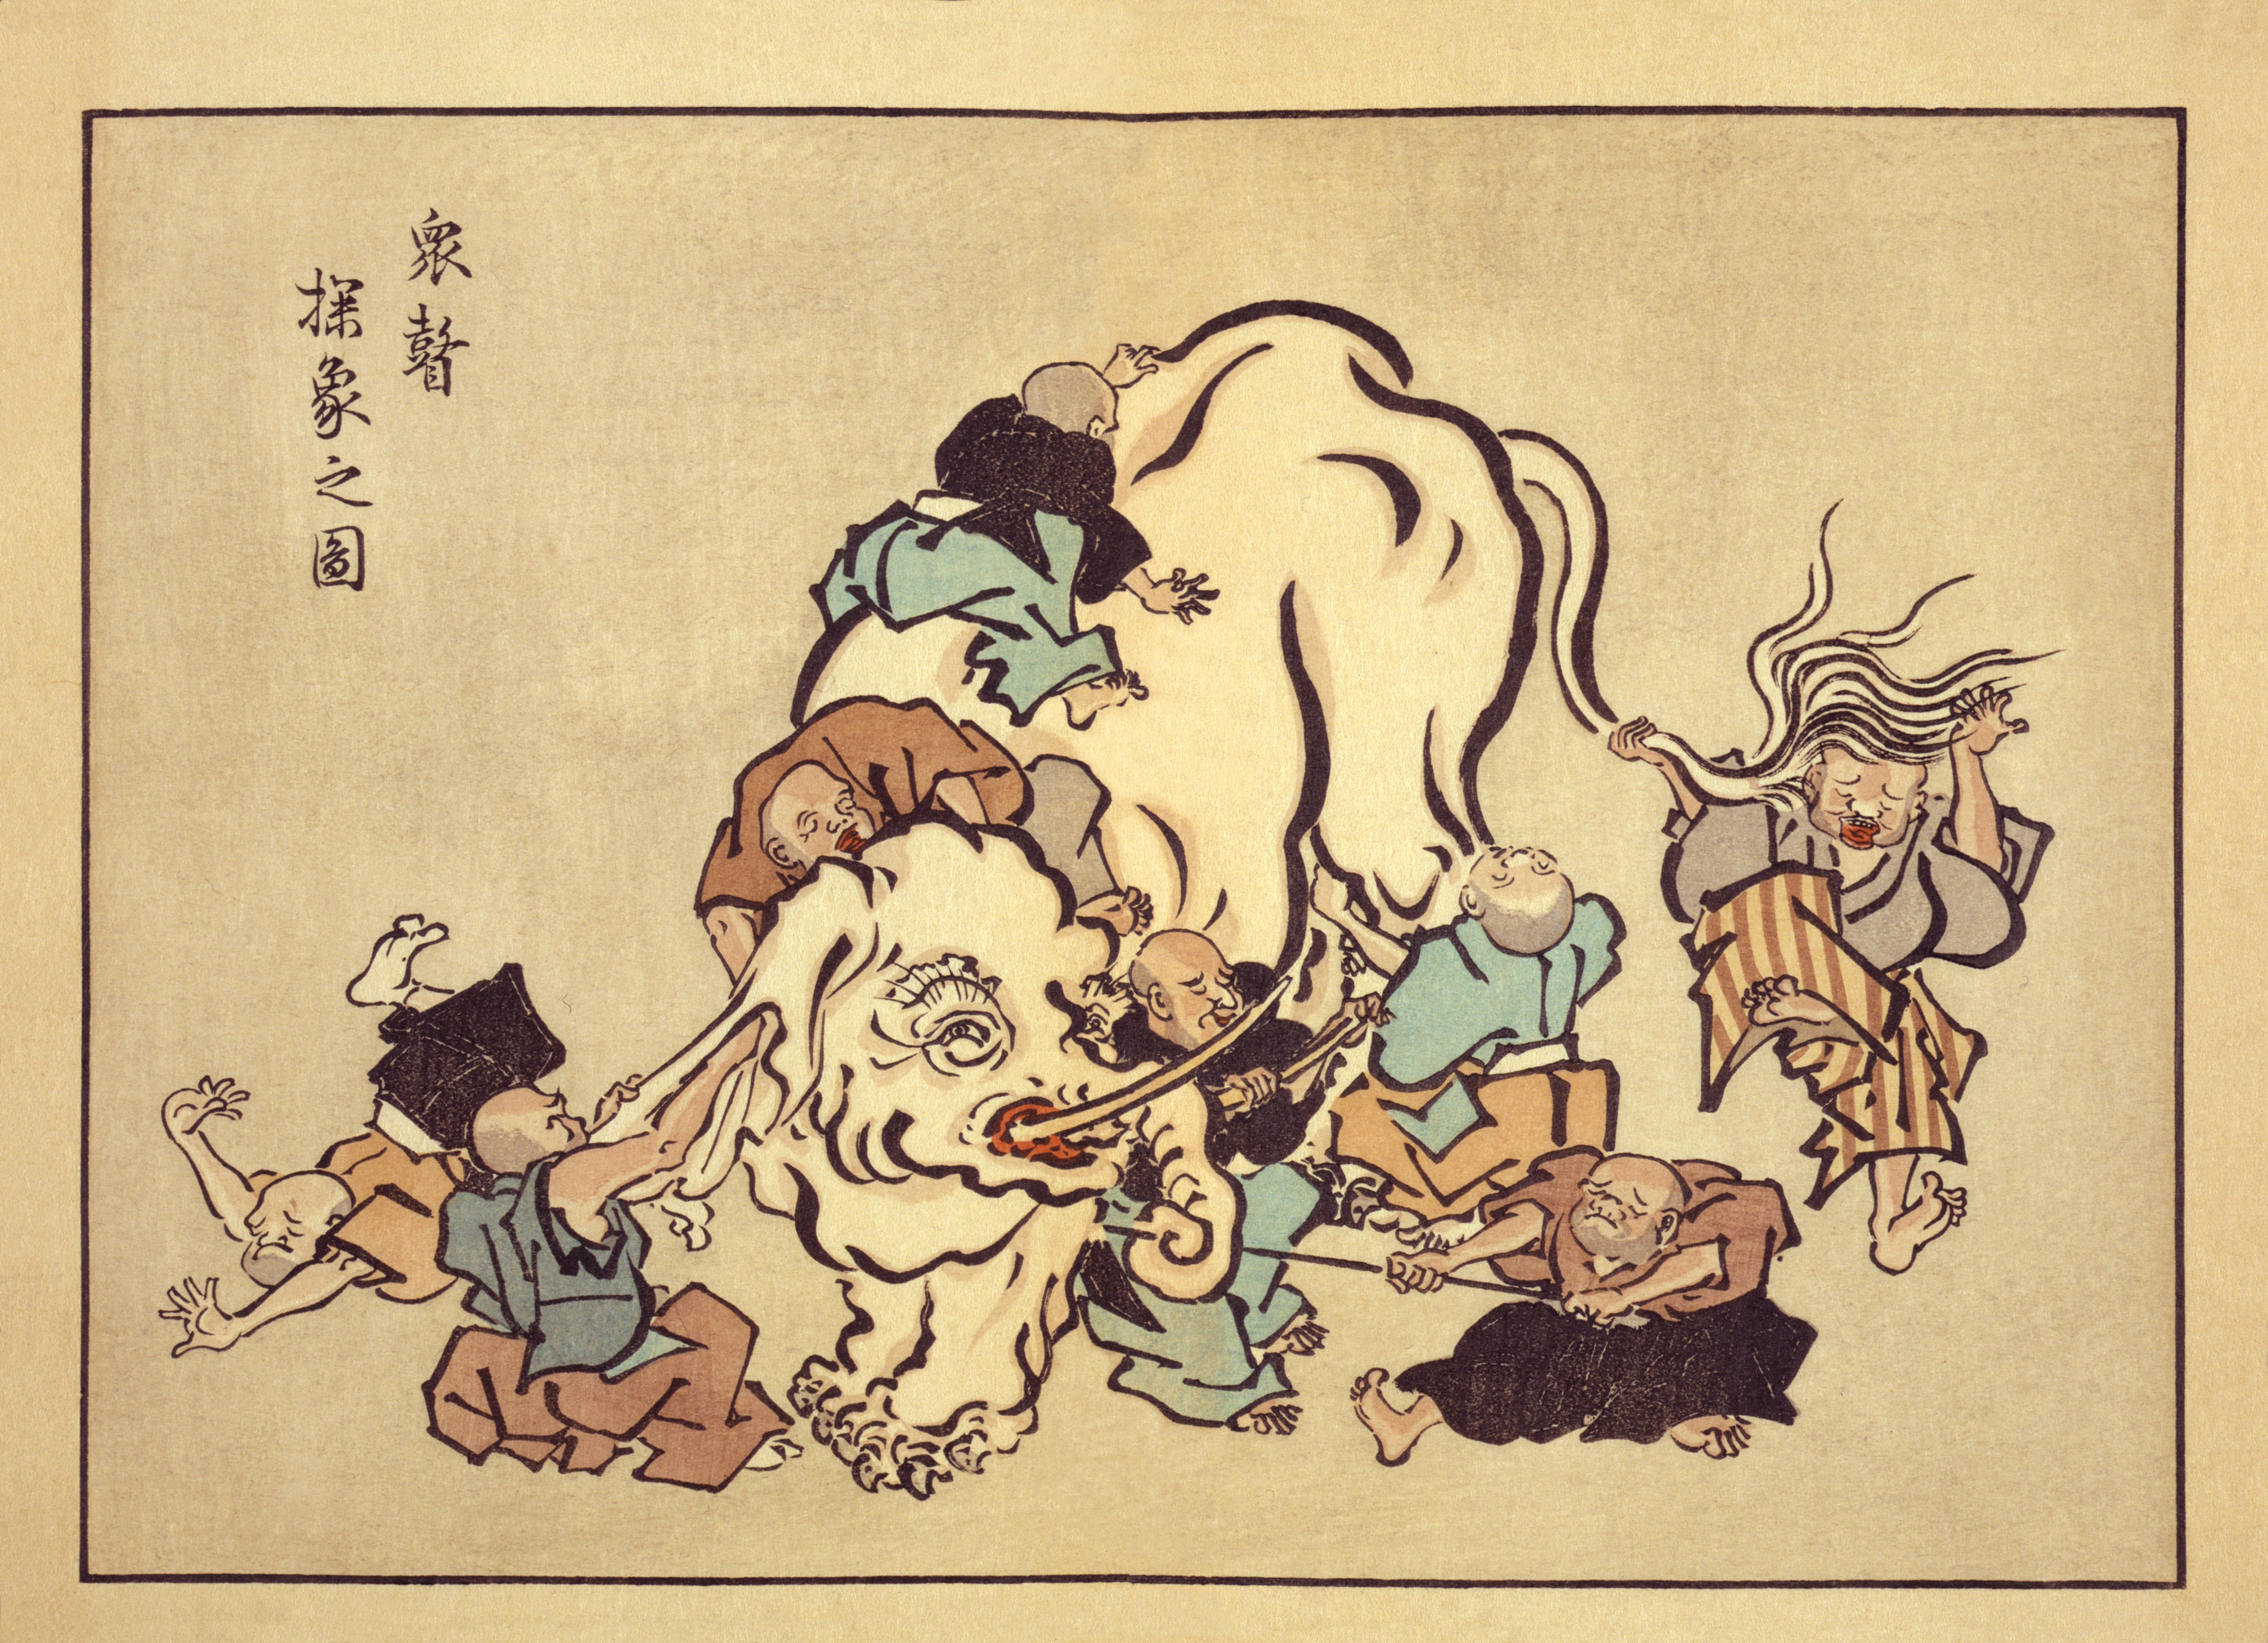
\includegraphics[width=0.6\textwidth]{elephant}\bigskip\bigskip\titlepage}
\frame{\tableofcontents}


\section[Kat.]{Kategorientheorie}

\subsection{Was sind Kategorien?}

\begin{frame}{Was sind Kategorien?}
  \hil{Kategorien} sind Ansammlungen von \hil{Objekten} zusammen mit
  \hil{Morphismen} zwischen ihnen.
  \bigskip

  {\centering\small\begin{tabular}{lll}
    \toprule
    Kategorie & Objekte & Morphismen \\\midrule
    $\mathrm{Set}$ & Mengen & Abbildungen \\
    $\mathrm{Vect}$ & Vektorräume & lineare Abbildungen \\
    $\mathrm{Hask}$ & Haskell-Typen & Haskell-Funktionen \\
    $\mathrm{Pkmn}$ & Pokémon & Entwicklungsprozesse \\
    $\mathrm{Cob}$ & Mannigfaltigkeiten & Kobordismen \\
    \bottomrule
  \end{tabular}\par}
  \bigskip

  Kategorientheorie stellt \hil{Beziehungen zwischen Objekten} statt etwaiger
  \hil{innerer Struktur} in den Vordergrund.
  \bigskip
  \pause

  Ein Objekt~$T$ ist genau dann \hil{terminal}, wenn es für jedes Objekt~$X$
  genau einen Morphismus $X \to T$ gibt.
  \par
\end{frame}


\subsection[Dualität]{Kategorielle Dualität}

\begin{frame}{Kategorielle Dualität}
  \begin{center}\begin{tabular}{r@{\quad vs.\quad}l}
    $f \circ g$ & $g \circ f$ \\
    $\leq$ & $\geq$ \\
    injektiv & surjektiv \\
    $\{\heartsuit\}$ & $\emptyset$ \\
    $\times$ & $\amalg$ \\
    ggT & kgV \\
    $\cap$ & $\cup$ \\
    Teilmenge & Faktormenge
  \end{tabular}\end{center}

  \hfill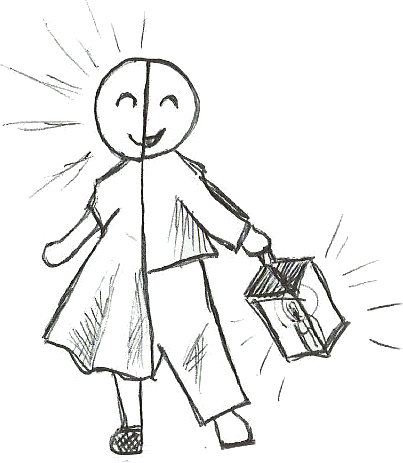
\includegraphics[width=0.3\textwidth]{dualitaet}
\end{frame}


\subsection[Anwendungen]{Anwendungen von Kategorientheorie}

\begin{frame}{Anwendungen von Kategorientheorie}
  \begin{itemize}
    \item Untersuchung von Dualität
    \item Systematische Sprache als Gerüst zum Denken
    \item Leitfaden, um richtige Definitionen zu formulieren
    \item Triviales wird trivialerweise trivial: \\
    \hil{Allgemeiner abstrakter Nonsens}
    \item Konzeptionelle Vereinheitlichung: \\
    \hil{Limiten, Kolimiten, adjungierte Funktoren}
  \end{itemize}

  \bigskip
  \centering
  \qquad\includegraphics[width=0.7\textwidth]{pizzaseminar}
  \par
\end{frame}


\section[Def.]{Elementartopoi}

\begin{frame}{Was sind Elementartopoi?}
  \hil{Elementartopoi} sind Kategorien mit so guten Eigenschaften, dass man
  "`in ihnen Mathe machen kann"'. Sie müssen besitzen:
  \begin{itemize}
    \item endliche Limiten: etwa $X \times Y$ und $\{ x \in X \,|\, f(x) = g(x) \}$
    \item interne Hom-Objekte
    \item einen Unterobjektklassifizierer: etwa $\Omega = \{ 0, 1 \}$
  \end{itemize}
  \bigskip

  \hil{Beispiele:}
  \begin{itemize}
    \item $\mathrm{Set}$, die Kategorie der Mengen
    \item $\mathrm{FinSet}$, die Kategorie der endlichen Mengen
    \item $\mathrm{Set}^2$, die Kategorie der Mengenpaare
    \item $\mathrm{Sh}(X)$, die Kategorie der Garben über einem Raum~$X$
    \item $\mathrm{Eff}(\mathcal{M})$, der ef{}fektive Topos zu einem Rechenmodell~$\mathcal{M}$
    \item Der Bohrtopos zu einem quantenmechanischem System~$A$
    \item Gödels und Cohens Topoi
  \end{itemize}
\end{frame}


\section[als Garbenkat.]{Topoi als Kategorien von Garben}

\begin{frame}{Topoi als Kategorien von Garben}
  Sei~$X$ ein Raum ($\mathbb{R}^n$, metrischer Raum, topologischer Raum,
  Örtlichkeit, Situs, Topos).
  \bigskip

  Eine \hil{Garbe} über~$X$ ist eine \hil{stetige Ansammlung von Mengen}, je
  eine für jeden Punkt von~$X$. Wir stellen uns Garben als \hil{veränderliche
  Mengen} vor.
  \bigskip

  \centering
  \small
  \begin{tabular}{ll}
    \toprule
    Raum $X$ & Kategorie der Garben über $X$ \\\midrule
    $\{\heartsuit\}$ & $\mathrm{Set}$ \\
    $\{\heartsuit,\varheart\}$ & $\mathrm{Set}^2$ \\
    $(\mathbb{N},\geq)$ & Kategorie der zeitabhängigen Mengen \\
    $\mathrm{Ring}^\mathrm{op}$ & Kategorie der Schemata (und allgemeinerer Räume) \\
    $\mathrm{Man}$ & Kategorie von mit Mnf. sondierbaren Räumen \\
    \bottomrule
  \end{tabular}
  \par
\end{frame}

\begin{frame}{Die Garbe der Kontinente}
  \centering
  \only<1>{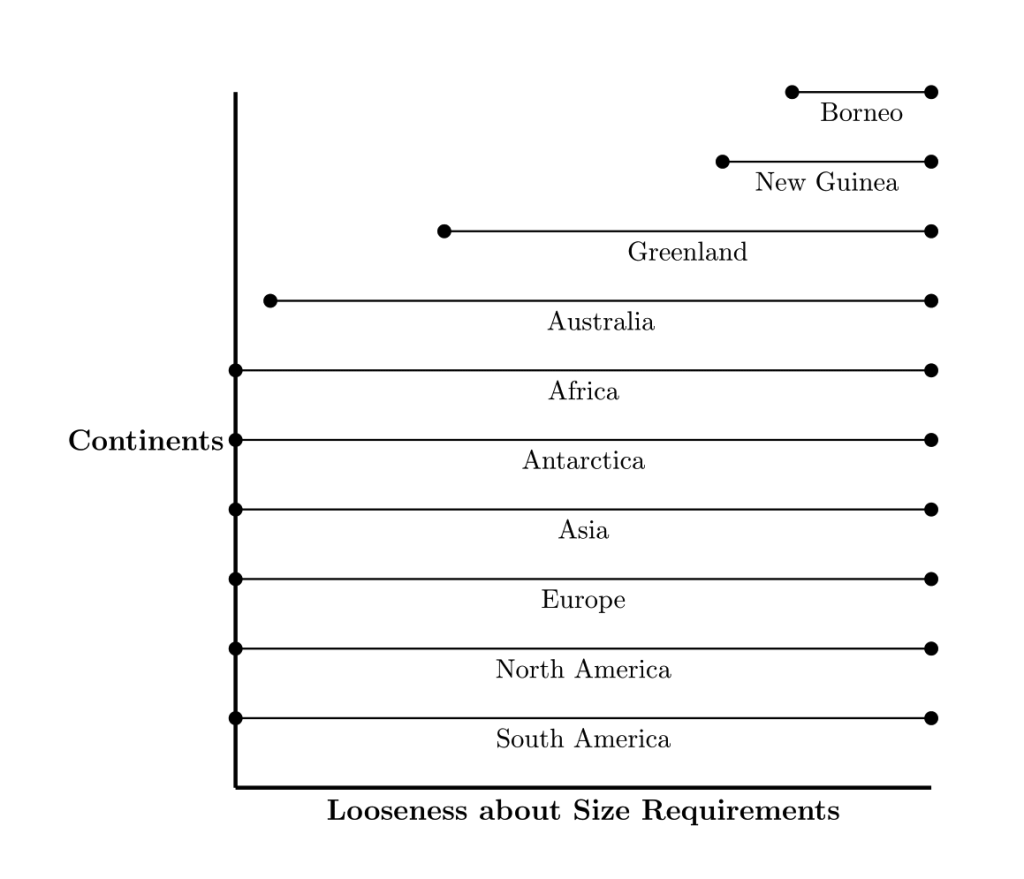
\includegraphics[width=0.8\textwidth]{continents1}}
  \only<2>{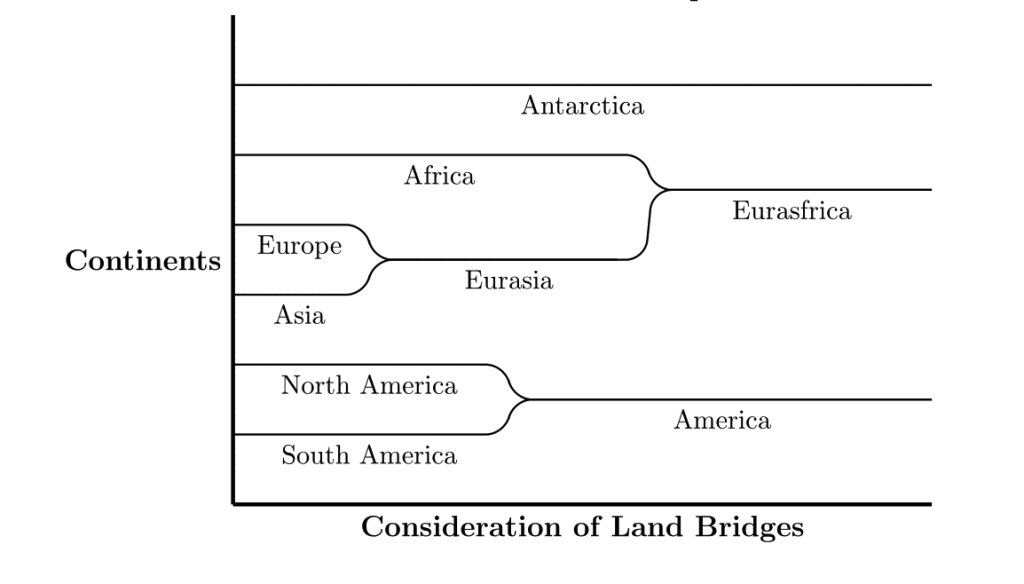
\includegraphics[width=0.8\textwidth]{continents2}}
  \par
\end{frame}


\section[als Räume]{Topoi als Räume}

\begin{frame}{Topoi als Räume}
  Wie bei konventionellen Räumen gibt es Konzepte wie
  \begin{itemize}
    \item \hil{Punkt eines Topos},
    \item \hil{offener Teil eines Topos},
    \item \hil{Untertopos},
    \item \hil{Garbe über einem Topos} (und ihre Kohomologie) und
    \item \hil{stetige Abbildung zwischen Topoi}.
  \end{itemize}
  Dabei stellen wir uns~$\mathrm{Sh}(X)$ grafisch wie~$X$ vor.

  \begin{itemize}
    \item Der Funktor~$X \mapsto \mathrm{Sh}(X)$ ist beinahe volltreu.
    \item Auch punktlose Topoi können nichttrivial sein: \\
    Topos der zufälligen 0/1-Folgen, \\
    Topos der Surjektionen~$\mathbb{N} \to \mathbb{R}$
    \item Topoi können riesig sein: Topos aller Gruppen
    \item Historische Motivation: der étale Topos eines Schemas
  \end{itemize}
\end{frame}


\section[als Universen]{Topoi als Alternativuniversen}

\begin{frame}[plain]
  \centering
  \vfill
  \only<1>{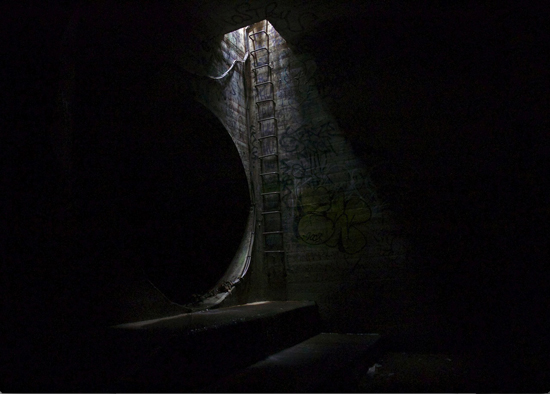
\includegraphics[width=0.9\textwidth]{leiter-der-angst}}
  \only<2>{
\includegraphics[width=0.9\textwidth]{baum-der-angst}}
  \par
\end{frame}
\addtocounter{framenumber}{-1}

\begin{frame}{Topoi als Alternativuniversen}
  Jeder Topos kommt mit einer \hil{internen Sprache} und lässt sich daher als
  \hil{Alternativuniversum}, in dem nicht unbedingt die üblichen Gesetze der
  Logik gelten, auffassen.
  \bigskip

  {\centering\small
  \begin{tabular}{ll}
    \toprule
    Topos~$\mathcal{E}$ & Bedeutung von~"`$\mathcal{E} \models \varphi$"' \\\midrule
    $\mathrm{Set}$ & Die Aussage $\varphi$ stimmt im üblichen Sinn. \\
    $\mathrm{Sh}(X)$ & Die Aussage $\varphi$ stimmt auf ganz~$X$. \\
    $\mathrm{Sh}(\mathbb{N},\geq)$ & Die Aussage~$\varphi$ stimmt zu jeder Zeit. \\
    $\mathrm{Eff}(\mathcal{M})$ & Es gibt einen berechenbaren Zeugen für $\varphi$. \\
    \bottomrule
  \end{tabular}\par}
  \bigskip

  Die Lingua franca aller Topoi ist \hil{konstruktive Mathematik}:
  \begin{itemize}
    \item kein Axiom vom ausgeschlossenen Dritten: $\varphi \vee \neg\varphi$
    \item kein Axiom der Doppelnegationselimination: $\neg\neg\varphi \Rightarrow \varphi$
    \item kein Auswahlaxiom
  \end{itemize}
\end{frame}

\begin{frame}{Konstruktive Mathematik?}
  Eine Zahl heißt genau dann \hil{rational}, wenn sie sich als Bruch zweier
  ganzer Zahlen schreiben lässt.
  \bigskip

  \hil{Satz.} Es gibt \hil{irrationale} Zahlen~$x$ und~$y$ sodass~$x^y$ rational ist.
  \bigskip

  \begin{center}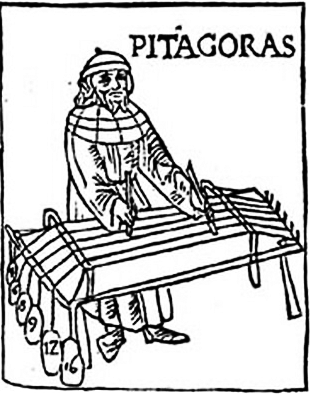
\includegraphics[scale=0.3]{pythagoras}\end{center}
\end{frame}

\begin{frame}{Beispiele}
  \centering
  In \hil{Gödels Topos} gilt: \\
  Es gibt keine Zwischenstufe zwischen $\mathbb{N}$ und $\mathbb{R}$.
  \bigskip

  In \hil{Cohens Topos} gilt: \\
  Es gibt eine Zwischenstufe zwischen $\mathbb{N}$ und $\mathbb{R}$.

  {\usebeamercolor[fg]{item}\hdashrule{\textwidth}{1pt}{3mm}\medskip}

  \pause

  Im \hil{glatten Topos} gilt: \\
  Es gibt infinitesimale Zahlen $\varepsilon$ mit $\varepsilon^2 = 0$, aber $\varepsilon \neq 0$.
  \bigskip

  \only<2>{
    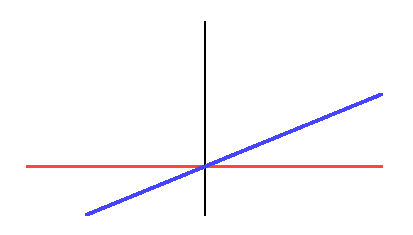
\includegraphics[height=0.3\textheight]{sdg-schnittverhalten1}
    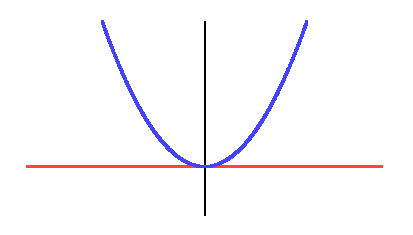
\includegraphics[height=0.3\textheight]{sdg-schnittverhalten2}
  }\pause

  Im \hil{ef{}fektiven Topos} gilt: \\
  Jede Funktion $\mathbb{N} \to \mathbb{N}$ ist durch ein Programm berechenbar.
  \bigskip
  \pause

  Im \hil{Zariski-Topos} gilt: \\
  Jede Funktion $R \to R$ ist ein Polynom.
  \bigskip
  \par
\end{frame}

\begin{frame}{Operationen mit Topoi}
  \begin{itemize}
    \item Jeder Topos besitzt einen \hil{kleinsten dichten Untertopos}.
    Dieser ist stets boolsch.
    \item Jeder Topos wird von einem boolschen Topos \hil{überdeckt}.
    \item Ist~$A$ ein Objekt eines Topos~$\mathcal{E}$, so enthält der
    Scheibentopos~$\mathcal{E}/A$ ein \hil{generisches Element} von~$A$.
    \item Ist~$\varphi$ eine Aussage der internen Sprache eines
    Topos~$\mathcal{E}$, so ist~$\mathcal{E}/\llbracket\varphi\rrbracket$ der
    \hil{größte offene Untertopos}, auf dem~$\varphi$ gilt.
    \item Unter gewissen Bedingungen kann man künstliche Injektionen und
    Surjektionen zu Topoi hinzufügen.
    \item Ist~$K$ ein Körper in einem Topos~$\mathcal{E}$, so lebt
    der \hil{separable Abschluss} von~$K$ in einem gewissen anderem Topos.
  \end{itemize}
\end{frame}


\section[als Theorien]{Topoi als Verkörperungen von Theorien}

\begin{frame}{Topoi als Theorien}
  Zu jeder \hil{geometrischen Theorie}~$T$ gibt es den Topos~$\mathrm{Set}[T]$
  der \hil{Modelle} von~$T$. Beispiele:

  \begin{itemize}
    \item Topos der Gruppen
    \item Topos der Ringe und sein Untertopos der lokalen Ringe
    \item Topos der Mengen
    \item Topos der Intervalle ($\simeq \mathrm{sSet}$)
  \end{itemize}

  In $\mathrm{Set}[T]$ lebt das \hil{generische Modell} von~$T$.
  \begin{itemize}
    \item Jedes Modell von~$T$ ist Rückzug des generischen Modells
    und erbt all dessen geometrische Eigenschaften.
    \item Quotiententheorien führen zu Untertopoi.
    \item Jeder Topos ist der Topos der Modelle einer Theorie.
    \item Verschiedene Theorien können äquivalente Topoi geben!
  \end{itemize}
\end{frame}


\section[]{Wieso sich mit Topoi befassen?}

{\usebackgroundtemplate{\begin{minipage}{\paperwidth}\vspace*{4.95cm}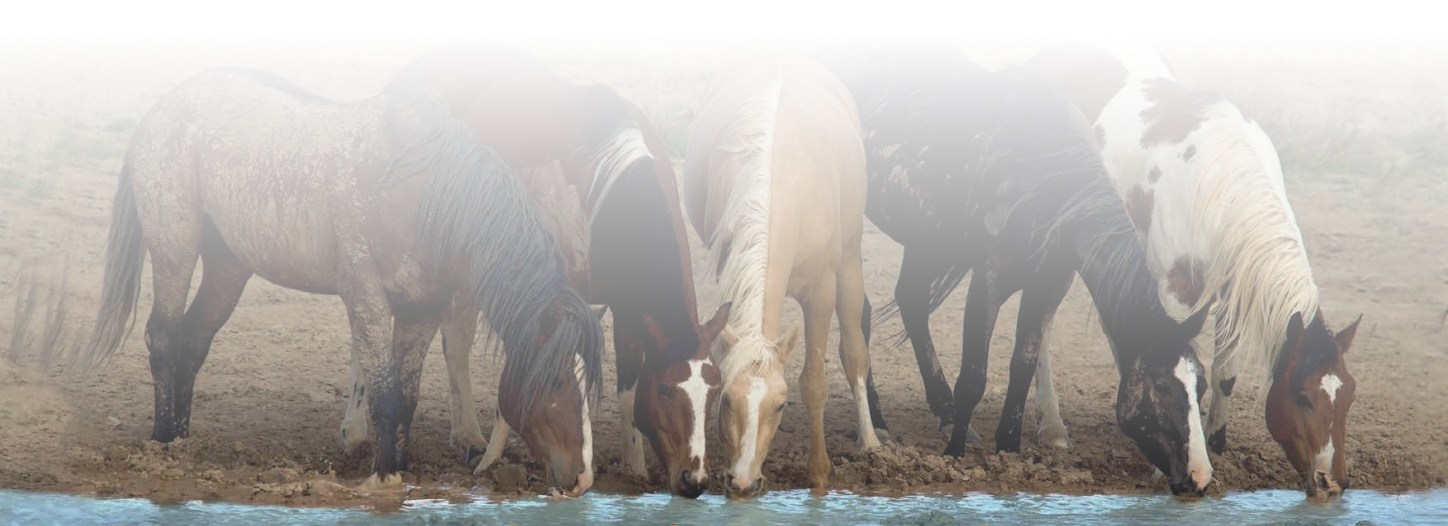
\includegraphics[width=\paperwidth]{topos-horses}\end{minipage}}
\begin{frame}{Wieso sich mit Topoi befassen?}
  Weil sie \ldots
  \begin{itemize}
    \item existieren,
    \item einen Beitrag zur Philosophie der Mathematik leisten,
    \item das Studium kurioser Traumaxiome ermöglichen,
    \item gewisse Konzepte vergegenständlichen können,
    \item ein flexibleres Raumkonzept bieten,
    \item \ \\[-1.2em]\mbox{Querverbindungen innerhalb der Mathematik herstellen und}
    \item mathematische Probleme vereinfachen können:

    für jede Situation den passenden Topos.
  \end{itemize}
\end{frame}}

\end{document}
